% THIS IS AN EXAMPLE DOCUMENT FOR VLDB 2012
% based on ACM SIGPROC-SP.TEX VERSION 2.7
% Modified by  Gerald Weber <gerald@cs.auckland.ac.nz>
% Removed the requirement to include *bbl file in here. (AhmetSacan, Sep2012)
% Fixed the equation on page 3 to prevent line overflow. (AhmetSacan, Sep2012)

\documentclass{vldb}
\usepackage{graphicx}
\graphicspath{ {images/} }
\usepackage{balance}  % for  \balance command ON LAST PAGE  (only there!)


\begin{document}

% ****************** TITLE ****************************************

\title{ Performance Evaluation of Stream Data Processing Systems}

% possible, but not really needed or used for PVLDB:
%\subtitle{[Extended Abstract]
%\titlenote{A full version of this paper is available as\textit{Author's Guide to Preparing ACM SIG Proceedings Using \LaTeX$2_\epsilon$\ and BibTeX} at \texttt{www.acm.org/eaddress.htm}}}

% ****************** AUTHORS **************************************

% You need the command \numberofauthors to handle the 'placement
% and alignment' of the authors beneath the title.
%
% For aesthetic reasons, we recommend 'three authors at a time'
% i.e. three 'name/affiliation blocks' be placed beneath the title.
%
% NOTE: You are NOT restricted in how many 'rows' of
% "name/affiliations" may appear. We just ask that you restrict
% the number of 'columns' to three.
%
% Because of the available 'opening page real-estate'
% we ask you to refrain from putting more than six authors
% (two rows with three columns) beneath the article title.
% More than six makes the first-page appear very cluttered indeed.
%
% Use the \alignauthor commands to handle the names
% and affiliations for an 'aesthetic maximum' of six authors.
% Add names, affiliations, addresses for
% the seventh etc. author(s) as the argument for the
% \additionalauthors command.
% These 'additional authors' will be output/set for you
% without further effort on your part as the last section in
% the body of your article BEFORE References or any Appendices.

\numberofauthors{8} %  in this sample file, there are a *total*
% of EIGHT authors. SIX appear on the 'first-page' (for formatting
% reasons) and the remaining two appear in the \additionalauthors section.

%\author{
% You can go ahead and credit any number of authors here,
% e.g. one 'row of three' or two rows (consisting of one row of three
% and a second row of one, two or three).
%
% The command \alignauthor (no curly braces needed) should
% precede each author name, affiliation/snail-mail address and
% e-mail address. Additionally, tag each line of
% affiliation/address with \affaddr, and tag the
% e-mail address with \email.
%
% 1st. author
%\alignauthor
%Ben Trovato\titlenote{Dr.~Trovato insisted his name be first.}\\
%   \affaddr{Institute for Clarity in Documentation}\\
%   \affaddr{1932 Wallamaloo Lane}\\
%   \affaddr{Wallamaloo, New Zealand}\\
%   \email{trovato@corporation.com}
%% 2nd. author
%\alignauthor
%G.K.M. Tobin\titlenote{The secretary disavows
%any knowledge of this author's actions.}\\
%   \affaddr{Institute for Clarity in Documentation}\\
%   \affaddr{P.O. Box 1212}\\
%   \affaddr{Dublin, Ohio 43017-6221}\\
%   \email{webmaster@marysville-ohio.com}
%% 3rd. author
%\alignauthor Lars Th{\Large{\sf{\o}}}rv{$\ddot{\mbox{a}}$}ld\titlenote{This author is the
%one who did all the really hard work.}\\
%   \affaddr{The Th{\large{\sf{\o}}}rv{$\ddot{\mbox{a}}$}ld Group}\\
%   \affaddr{1 Th{\large{\sf{\o}}}rv{$\ddot{\mbox{a}}$}ld Circle}\\
%   \affaddr{Hekla, Iceland}\\
%   \email{larst@affiliation.org}
%\and  % use '\and' if you need 'another row' of author names
%% 4th. author
%\alignauthor Lawrence P. Leipuner\\
%   \affaddr{Brookhaven Laboratories}\\
%   \affaddr{Brookhaven National Lab}\\
%   \affaddr{P.O. Box 5000}\\
%   \email{lleipuner@researchlabs.org}
%% 5th. author
%\alignauthor Sean Fogarty\\
%   \affaddr{NASA Ames Research Center}\\
%   \affaddr{Moffett Field}\\
%   \affaddr{California 94035}\\
%   \email{fogartys@amesres.org}
%% 6th. author
%\alignauthor Charles Palmer\\
%   \affaddr{Palmer Research Laboratories}\\
%   \affaddr{8600 Datapoint Drive}\\
%   \affaddr{San Antonio, Texas 78229}\\
%   \email{cpalmer@prl.com}
%}
% There's nothing stopping you putting the seventh, eighth, etc.
% author on the opening page (as the 'third row') but we ask,
% for aesthetic reasons that you place these 'additional authors'
% in the \additional authors block, viz.
\additionalauthors{Additional authors: John Smith (The Th{\o}rv\"{a}ld Group, {\texttt{jsmith@affiliation.org}}), Julius P.~Kumquat
(The \raggedright{Kumquat} Consortium, {\small \texttt{jpkumquat@consortium.net}}), and Ahmet Sacan (Drexel University, {\small \texttt{ahmetdevel@gmail.com}})}
\date{30 July 1999}
% Just remember to make sure that the TOTAL number of authors
% is the number that will appear on the first page PLUS the
% number that will appear in the \additionalauthors section.


\maketitle

\begin{abstract}
Over the past years, Stream data processing is gaining compelling attention both in industry and in academia due to its wide range of applications in various use-cases. To fulfil the need for efficient and high performing  Big data analytics, numerous open source stream data processing systems were developed. Processing data with high throughput while retaining low latency is key performance indicator for such systems. In this paper, we propose a benchmarking system to evaluate the performance of stream  data processing systems, Storm, Spark and Flink  in terms of indicators shown above. More specifically, the latency of windowed aggregation and windowed join operators is evaluated jointly  with the throughput of a system. 
\end{abstract}




\section{Introduction}
Streaming data processing has been gaining significant attention due to its wide range of uses in Big data analytics. The main reason is that processing big volumes of data periodically is not enough anymore and data has to be processed fast to enable fast adaptation and reaction to changed conditions. Several engines are widely adopted and supported by open source community, such as Apache Storm \cite{toshniwal2014storm}, Apache Spark  \cite{zaharia2012discretized} , Apache Flink \cite{carbone2015apache} and etc.

\section{Related work}

\section{PRELIMINARY AND BACKGROUND}
\subsection{Storm}
general info, windowing, partitioning, join.
\subsection{Spark}
general info, windowing, partitioning, join.
\subsection{Flink}
general info, windowing, partitioning, join.


\section{Benchmark system design}
We keep overall design of benchmark simple and akin to the systems under to be tested.  
The stream data processing system connects to predefined number of socket input data sources. Each input data source has its own data generator and queue where tuples are put after generation. When the stream data processing system pulls  data from socket server, serving thread sends the data from queue rather than  directly from data generator. 

Figure \ref{fig_design} shows the overall intuition of the benchmark system.Firstly, the data generator, at the left side of the figure, spawns the tuples and appends the current timestamp as a separate field. Secondly, the generated tuples wait in queue until the stream data processing system pulls them. Queue is based on FIFO semantics. Thirdly, the stream data processing system combines the tuples from different sockets by uniting streams. Depending on the nature of operator to be tested, there can be several unions of streams. For example, windowed aggregation is single input stream operator but join operator accepts two streams as an input. Fourthly, the operator to be tested computes the data in windows. In our case, we test windowed aggregation and windowed join operators. Finally, the next operator calculates the latency of a tuple by subtracting event timestamp from current timestamp.

Proper handling tuple's timestamp fields while joining or aggregating is crucial. Lets say, $t_{a}^{m}$ is a tuple from socket stream $a$, residing in window $m$ and $t_{a}^{m}$ denote the value of $k{th}$ field. 
restrictions..

\begin{figure*}[h]
\caption{Design of benchmark system.}
\centering
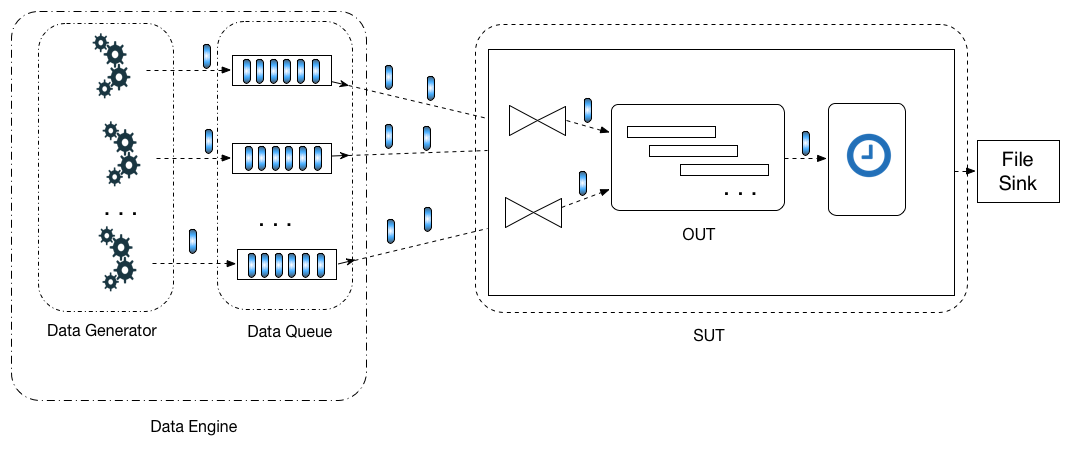
\includegraphics[width=1\textwidth]{system_design}
\label{fig_design}
\end{figure*}


\subsection{Key Performance Indicators}
\section{Evaluation}
\subsection{Keyed Windowed Aggregations}
scale up/down

window size increase/decrease

batch siez increase/decrease

\subsection{Joins}
same as above
\section{Conclusions}
%\end{document}  % This is where a 'short' article might terminate

% ensure same length columns on last page (might need two sub-sequent latex runs)
\balance

%ACKNOWLEDGMENTS are optional
\section{Acknowledgments}


% The following two commands are all you need in the
% initial runs of your .tex file to
% produce the bibliography for the citations in your paper.
\bibliographystyle{abbrv}
\bibliography{vldb_sample}  % vldb_sample.bib is the name of the Bibliography in this case
% You must have a proper ".bib" file
%  and remember to run:
% latex bibtex latex latex
% to resolve all references

\subsection{References}
Generated by bibtex from your ~.bib file.  Run latex,
then bibtex, then latex twice (to resolve references).

%APPENDIX is optional.
% ****************** APPENDIX **************************************
% Example of an appendix; typically would start on a new page
%pagebreak

\begin{appendix}
You can use an appendix for optional proofs or details of your evaluation which are not absolutely necessary to the core understanding of your paper. 


\end{appendix}



\end{document}
